\chapter{Discrete element method}

Discrete element method (DEM) is a numerical tool used to model discrete systems by
solving Newton's equations of motion on each particle in the system. It also
allows to model continuous systems by discretizing into particles.


\section{Introduction}
\label{sec:introduction}

Let's first discuss a real life example before discussing the algorithm of
DEM.\@ Consider sand, sand consists of many discrete particles which has mass, a
definite shape and other properties. We want to know the dynamics of sand
flowing through various bodies such as a hopper, hour-glass or a filter. One way
of modelling such system is to assume the sand to be a continuum and by
conservation laws we can solve for various macroscopic properties such as
stress, strain etc, just like solving for a fluid or solid.

Unfortunately, a system like sand, behaves differently at different places. As
an example consider the behaviour of sand flowing under gravity in an hourglass
(see fig \ref{fig:hourglass}) \footnote{taken from
  \href{https://www.istockphoto.com/in/videos/hourglass?sort=mostpopular&offlinecontent=include&phrase=hourglass}
  {istockphoto}.}  and second example of particles getting jammed in a hopper
(see fig \ref{fig:hopper_jam} \footnote{taken from
  \href{http://webhome.phy.duke.edu/~jt41/research.html}{Junyao Tang's Home
    Page}}). We can observe in hourglass example as the sand flows like fluid
while it passes through the opening. By seeing this part and considering to
model the system as continuum would be would be a choice. But as soon as as it
hits the ground, rather than behaving like a fluid and flowing towards the wall,
it forms into a mountain. In the second example it is even more ambiguous,
rather than flowing out completely particles gets jammed.


\begin{figure}[h]
  \begin{subfigure}{0.5\textwidth}
    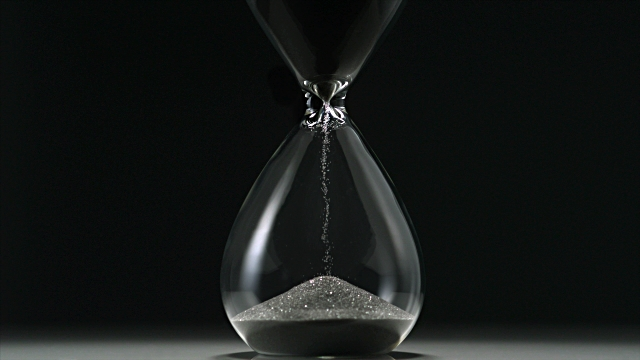
\includegraphics[width=0.9\linewidth, height=5cm]{dem/doc_images/hourglass}
    \caption{Sand exhibiting different behaviour in an hourglass}
    \label{fig:hourglass}
  \end{subfigure}
  \begin{subfigure}{0.5\textwidth}
    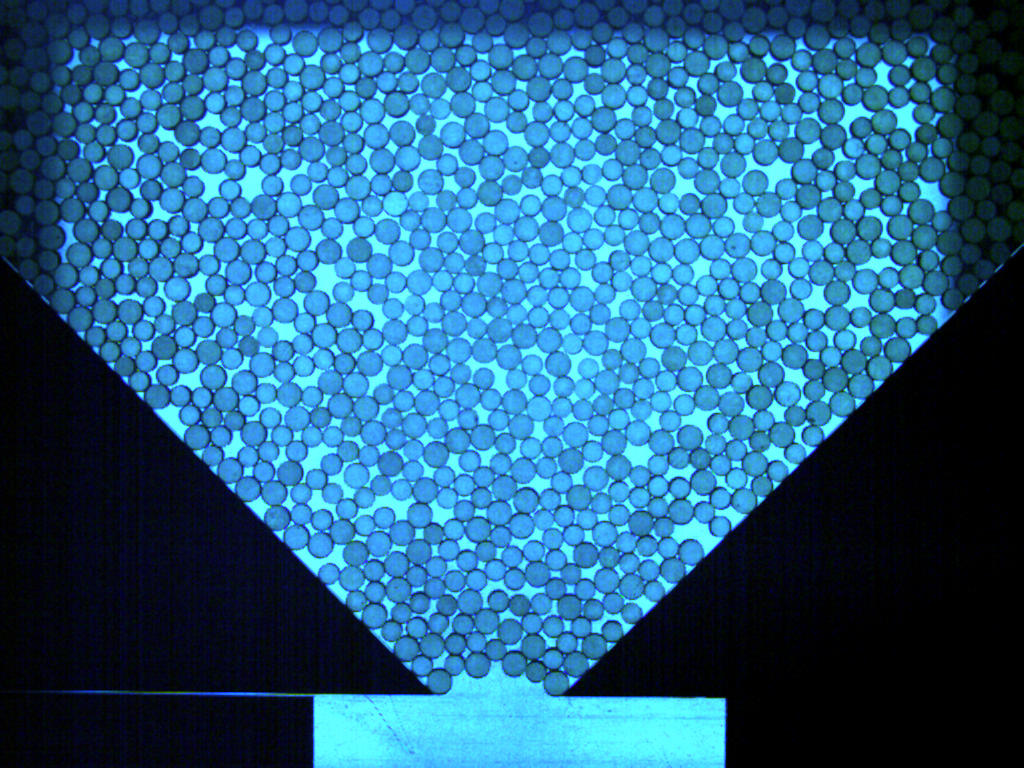
\includegraphics[width=0.9\linewidth, height=5cm]{dem/doc_images/hopper_jam}
    \caption{Particles jammed in a hopper}
    \label{fig:hopper_jam}
  \end{subfigure}

  \caption{Unexpected behaviour of a system with discrete particles}
  \label{fig:dem_introduction}
\end{figure}

In 1979 \citeauthor{Cundall_1979} introduced DEM to model such system. They
models the system using many discrete particles having specific shape, mass,
material properties and which interact at surfaces, and their dynamics is
captures using Newton's law of motion.

In the present chapter we will discuss in detail of DEM implementation. In the
next section the steps involved to set up a DEM simulation is discussed. In the
later section contact force models are discussed. After that the simulation
parameters, such as spring stiffness, damping coefficient and other parameters
which govern the simulation are discussed.


\section{DEM algorithm}
\label{sec:dem-algorithm}

As we discussed in the previous section about assuming the system to be composed
of discrete particles with mass, shape and other mechanical properties. Since it
is a particle with definite mass we can compute the dynamics of such particle
using the Newton's 2nd law.


\begin{gather}
  \label{eq:dem:equations_of_motion}
  m_i \, \dv{\vec{x}_i}{t} = \vec{f}_i\\
  J_i \, \dv{\vec{\dot{\omega}}_i}{t} = \vec{M}_i\\
  \vec{f}_i = m_i \,\vec{g} + \sum_i^N \vec{f}_{ij}^c + \vec{f}_{ext}\\
  \vec{M}_i = \vec{M}^r + \vec{M}^c
\end{gather}
where $\vec{f}_i$ and $\vec{M}_i$ are the force and moment acting on particle
$i$. Further these forces are decomposed into gravity ($m_i \, \vec{g}$),
contact force due to other particle $j$ ($\vec{f}_{ij}$ force on i due to j) and
any other external force ($\vec{f}_{ext}$).

A visual representation of these forces is given in figure
~\ref{fig:basic_forces_dem}.

\begin{figure}[htb]
  \centering
  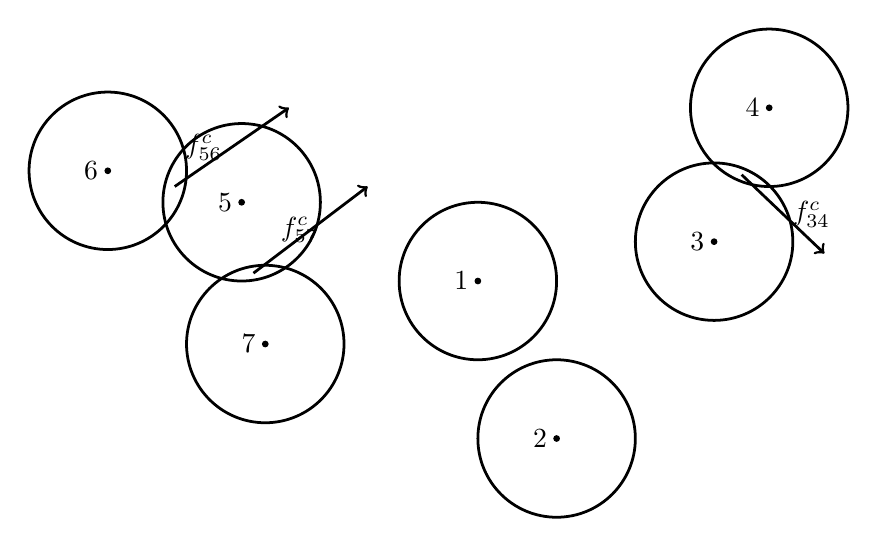
\begin{tikzpicture}
    % ---------------------------------------------
    % two spheres faraway
    \draw[line width=1pt] (0, 0) circle[radius=1];
    \draw[fill] (0,0) circle[radius=1pt];
    \node[left] at (0, 0) {$1$};
    \draw[line width=1pt] (1, -2) circle[radius=1];
    \draw[fill] (1, -2) circle[radius=1pt];
    \node[left] at (1, -2) {$2$};

    % ---------------------------------------------
    % two spheres interacting
    \draw[line width=1pt] (3, 0.5) circle[radius=1];
    \draw[fill] (3, 0.5) circle[radius=1pt];
    \node[left] at (3, 0.5) {$3$};
    \draw[line width=1pt] (3.7, 2.2) circle[radius=1];
    \draw[fill] (3.7, 2.2) circle[radius=1pt];
    \node[left] at (3.7, 2.2) {$4$};
    % draw force vector on particle 3
    \draw[->, line width=1pt] (3.35, 1.35) -- (4.4, 0.35);
    \node[right] at (3.875, 0.85) {$f^c_{34}$};

    % ---------------------------------------------
    % three spheres interacting
    \draw[line width=1pt] (-3, 1.0) circle[radius=1];
    \node[left] at (-3, 1.0) {$5$};
    \draw[fill] (-3, 1.0) circle[radius=1pt];

    \draw[line width=1pt] (-4.7, 1.4) circle[radius=1];
    \node[left] at (-4.7, 1.4) {$6$};
    \draw[fill] (-4.7, 1.4) circle[radius=1pt];

    \draw[line width=1pt] (-2.7, -0.8) circle[radius=1];
    \node[left] at (-2.7, -0.8) {$7$};
    \draw[fill] (-2.7, -0.8) circle[radius=1pt];

    % find forces on 5 due to 6 and 7
    \draw[->, line width=1pt] (-3.85, 1.2) -- (-2.4, 2.2);
    \node[left] at (-3.125, 1.7) {$f^c_{56}$};
    \draw[->, line width=1pt] (-2.85, 0.1) -- (-1.4, 1.2);
    \node[right] at (-2.625, 0.65) {$f^c_{57}$};

  \end{tikzpicture}
  \caption{Forces acting on particles due to contact}
  \label{fig:basic_forces_dem}
\end{figure}

The contact force ($f^c$) acts at the contact point of the two spheres. This
force is computed using various contact force models, such as linear spring
dashpot model (LSD) or a nonlinear model, Hertz model.


\section{Contact force modelling}
\label{sec:cont-force-modell}

In the previous section we saw interaction of spheres and forces acting on each
sphere. To make our life simple let's consider two spheres $i$ and $j$, to model
the contact force ($f^c$). Let $n_{ij}$ be the normal vector passing from $j$ to
$i$. $c$ is the contact point. $v_i$ and $v_j$ are velocities of particles $i$ and $j$ respectively. This
contact force can further be resolved into normal and tangential direction (see
fig \ref{fig:two_particles_collide}).
\begin{equation}
  f^c_{ij} = f^n \vec{n} + f^t \vec{t}
\end{equation}
Each force direction can be further decomposed into a conservative and a damping component.
Let's first discuss the normal force.

\begin{figure}[htb]
  \centering
  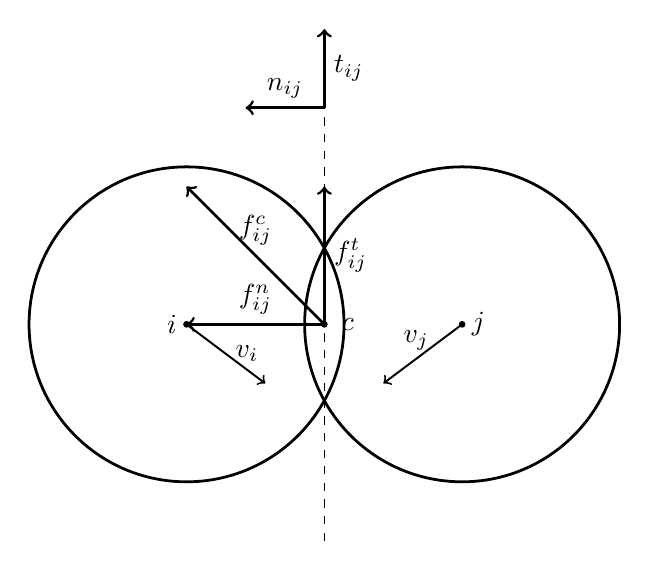
\begin{tikzpicture}
    % ---------------------------------------------
    \draw[line width=1pt] (0, 0) circle[radius=2];
    \draw[fill] (0,0) circle[radius=1pt];
    \node[left] at (0, 0) {$i$};
    \draw[line width=1pt] (3.5, 0) circle[radius=2];
    \draw[fill] (3.5, 0) circle[radius=1pt];
    \node[right] at (3.5, 0) {$j$};

    % draw normal vector
    \draw[dashed] (1.75, -2.75) -- (1.75, 3.75);
    \draw[->, line width=1pt] (1.75, 2.75) -- (0.75, 2.75);
    \node[above] at (1.25, 2.75) {$n_{ij}$};
    \draw[->, line width=1pt] (1.75, 2.75) -- (1.75, 3.75);
    \node[right] at (1.75, 3.25) {$t_{ij}$};

    % draw force components
    \draw[->, line width=1pt] (1.75, 0) -- (0.0, 1.75);
    \node[above] at (0.875, 0.875) {$f^c_{ij}$};
    \draw[->, line width=1pt] (1.75, 0) -- (0.0, 0);
    \node[above] at (0.875, 0) {$f^n_{ij}$};
    \draw[->, line width=1pt] (1.75, 0) -- (1.75, 1.75);
    \node[right] at (1.75, 0.875) {$f^t_{ij}$};

    % contact point
    \draw[fill] (1.75, 0) circle[radius=1pt];
    \node[right] at (1.85, 0) {$c$};

    % velocities
    \draw[->, line width=0.7pt] (0, 0) -- (1., -.75);
    \node[right] at (0.5, -0.375) {$v_i$};
    \draw[->, line width=0.7pt] (3.5, 0) -- (2.5, -.75);
    \node[left] at (3.2, -0.20) {$v_j$};

  \end{tikzpicture}
  \caption{Two particles colliding}
  \label{fig:two_particles_collide}
\end{figure}

\subsection{Normal contact force}
\label{sec:normal-contact-force}

Simplest way of modelling normal contact force is by linear spring dashpot
model, given by,


\begin{equation*}
  \label{eq:delta_overlap}
  f^n = k_n \, \delta + \gamma_n v_n
\end{equation*}
where $v_n = -v_{ij}\cdot \vec{n}$ and $\delta$ is overlap amount.

\begin{equation*}
  \delta = a_i + a_j - \norm{\vec{r}_i - \vec{r}_j}
\end{equation*}
$k_n$ is the spring stiffness and is an ad hoc value which is compromised with
the overlap amount. $\gamma_n$ is damping coefficient evaluated using
coefficient of restitution.


\subsection{Tangential force}
\label{sec:tangential-force}

Tangential force is divided into two phases, one is sticking and the other one
is sliding. Sticking is when the tangential force between two particles is less
than the Coulomb friction, in this condition particles at contact point won't
move, rather the centers of the particles will move elastically. In sliding
motion, the tangential force exceeds the friction force and the particles starts
to slide. In sliding condition the tangential force is bounded by Coulomb
frictional force.

Similar to normal component tangential component is also composed
of a conservative and non conservative part. Unlike conservative normal contact
force, conservative part in tangential direction is complicated. At a given time
step, in normal force law one computes the overlap amount at that instant and
uses it for force, but in tangential direction one needs to keep track of the
spheres which are in overlap and increment those springs elongation. The force
law is given by

\begin{equation}
  \label{eq:tangential_force_spring_damping}
  \vec{f}_{t0} = -k_t \, \vec{\delta}_t - \gamma_t \, \vec{v}_t
\end{equation}


\begin{equation*}
  \vec{\delta}_t = \vec{\delta}_t + \vec{v}_t \, dt
\end{equation*}

As we can observe from equation \ref{eq:tangential_force_spring_damping},
the conservative part is in the opposite direction of the elongation similar
to the normal conservative part. The non conservative part is in the opposite
direction of the tangential velocity which will reduce the energy of the
particle.

Once we compute the tangential force from the springs elongation, we compare it
with maximum allowed tangential force, i.e., static friction $\mu_s \, f_n$ if
the tangential force exceeds static friction then the particles start to slide
the tangential force is adjusted to sliding friction.

\begin{equation}
  \label{eq:tangential_force_spring_damping}
  f_t = \max(\norm{f_{t0}}, \mu_s f_n) \vec{t}
\end{equation}
where $\vec{t}$ is the direction of $\frac{\vec{f}_{t0}}{\norm{\vec{f}_{t0}}}$.



\section{Application to Rigid body simulation}
\label{sec:appl-rigid-body}

DEM can be applied to rigid body simulation to evaluate the forces between rigid
bodies in collision. The modelling process starts by discretizing the rigid
bodies into particles (Fig~\ref{fig:rigid_body_particles}).
\footnote{Taken from Nvidia}
\begin{figure}[ht]
  \label{fig:rigid_body_particles}
  \centering
  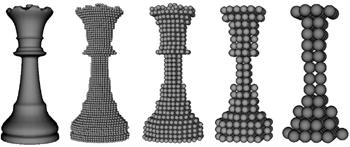
\includegraphics[width=0.9\linewidth, height=5cm]{dem/doc_images/grid_to_particles}
  \caption{Rigid body discretized as particles}
\end{figure}


The dynamics of rigid body are simulated using Newton's equations. Consider a
body ($I$) having discretized into $k$ particles. Let the moment of inertia of
such body at a given time step be $I_I$. In a simulation loop at every time step
forces on the particle are evaluated using SPH and DEM due to interaction with
other particles of fluid and solid phases and are saved in $\dv{\vec{v}_k}{t}$.
After evaluating forces on particles, these forces are transferred to the center
of mass of the rigid body as a resulting moment and force.

\begin{eqnarray}
  \label{eq:rigid_body_newton_equation}
  M_I \dv{\vec{V}_I}{t} &=& \sum_{k \in I} m_k \dv{\vec{v}_k}{t}\\
  I_I \dv{\vec{\Omega}_I}{t} &=& \sum_{k \in I} m_k (\vec{r}_k - \vec{R}_I) \cross \dv{\vec{v}_k}{t}
\end{eqnarray}
After evaluating the resultant moment at the center of mass of the body, the
moment of inertia is computed through which angular velocity at the next time
step is evaluated. Using the angular velocity at the center, the linear
velocities of the particles are evaluated and used to propagate the particle
positions to next time.


Drawbacks of such algorithm is to evaluate the moment of inertia at each and
every time step, which is costly. To overcome such operation one can use
rotation matrices. Detailed explanation can be found at
\href{https://www.cs.cmu.edu/~baraff/sigcourse/notesd1.pdf}{Baraff unconstrained
  dynamics}.

\section{Bonded Discrete element method}
\label{sec:bond-discr-elem}

\citeauthor*{Potyondy_2004} in extended DEM to model the deformation and
fracture of body. It follows bonding the particles with its neighbours using
springs (Fig~\ref{fig:bonded_dem}).


\begin{figure}
  \centering
  \caption{Particles bonded to neighbours}
  \label{fig:bonded_dem}
\end{figure}

%%

%%% Local Variables:
%%% mode: latex
%%% TeX-master: "../mainrep"
%%% End:

%  LocalWords:  Baraff
